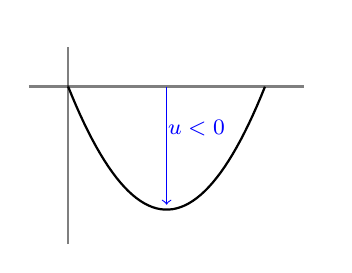
\begin{tikzpicture}
% Axis
\draw[thick,opacity=0.5] (-0.5,0)--(3,0) node[right]{$ $};
\draw[thick,opacity=0.5] (0,-2)--(0,0.5) node[above]{$ $};

\draw[samples=50, domain=0:2.5, thick] plot ({\x}, {\x*(\x - 2.5)});

\draw[->, blue] (1.25, 0) -- (1.25, -1.5) node [blue, right, pos=0.35, xshift=-3pt] {\footnotesize $u < 0$ };

\end{tikzpicture}
